\scanpage{40}
\mspage{19}
a) $S'\longrightarrow S^{\deleted{\unsure{'}}}$ surjectif, $\widetilde B'\longrightarrow\widetilde A^{\deleted{\unsure{'}}}$ \uline{bijectif}

b) \diagram{\begin{tikzcd}
I'\arrow[r,"\sim"]\arrow[d]&I\arrow[d]\\
S'\arrow[r]&S
\end{tikzcd}} commutatif

\margin{donc \diagram{\begin{tikzcd}
\widetilde B'\amalg I'\arrow[r,"\sim"]\arrow[d]&\widetilde A\amalg I\arrow[d]\\
S'\arrow[r]&S
\end{tikzcd}} est comm.}

c) $\forall\alpha\in S$, le sous-graphe $G'(\alpha)$ de $G'$ [formé des \deleted{\unsure{$S$}} $s'\in S'$ au dessus de $\alpha$, et des \deleted{flèches} arcs $a'\in\widetilde A'$ qui sont dans $\inserted{\widetilde C'=}\widetilde A'\setminus\widetilde B'$ (i.e. au dessus de $\operatorname{id}_\alpha$) et dont l'origine (donc l'extrémité aussi) est dans $S'_\alpha$], muni de \deleted{\unsure{$\widetilde A$}\unsure{ et }\unsure{$A$}} $I'_\alpha\inserted{\amalg\unsure{\widetilde B'_\alpha}}\longrightarrow S'_\alpha$ induit par $\inserted{\widetilde B'\amalg}I'\unsure{\to|{-}}S'$, et de $\gamma_\alpha:S'_\alpha\longrightarrow\mathbb N$ induit par $g':S'\unsure{\to|{-}}\mathbb N$, est un \uline{MD-graphe} \inserted{$\underline G'(\alpha)$} \deleted{\unsure{de type|de genre} $\unsure{g=g(\alpha)|(g_\alpha,\nu_\alpha)}$\unsure{, i.e.}}, i.e. il est \uline{connexe}, \deleted{[NB il \unsure{satisfait automatiquement}} \inserted{et [il satisfait \unsure{tous}}\deleted{\unsure{les}} \inserted{les} conditions de rigidité relatives aux sommets $\beta$ tels que, \deleted{\unsure{$\alpha$}} $g'_\beta\in\{0,1\}$, à savoir que

\margin{\uline{NB} $\widetilde B'_\alpha$ est l'ens des $\vec a'\in\widetilde B'_\alpha$ dont l'origine se trouve dans $S'_\alpha$, i.e. dans $G'(\alpha)$, donc $\widetilde B'_\alpha\xrightarrow{\sim}\widetilde A_\alpha$}

\figure{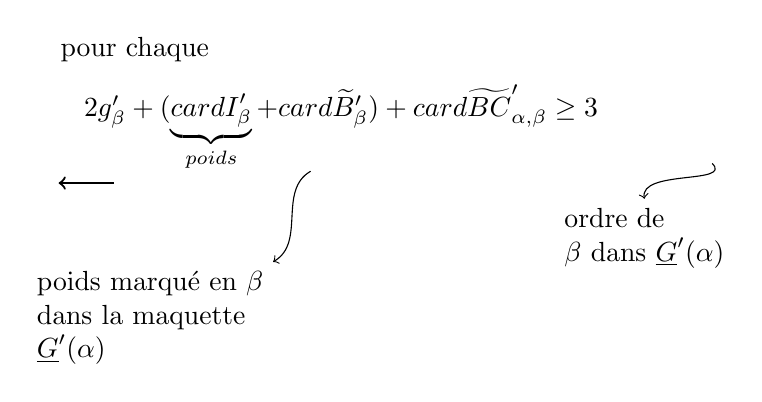
\begin{tikzpicture}[x=1cm,y=1cm]
\node[anchor=west] (eq) at (0,0) {$2g'_\beta+(\underbrace{\operatorname{card}I'_\beta}_{\deleted{\unsure{poids}}}\inserted{+\operatorname{card}\widetilde B'_\beta)}+\operatorname{card}\widetilde{\deleted{B}\inserted{C}}'_{\deleted{\unsure{\alpha}},\beta}\geq3$};
\node[anchor=north west,align=left] (mark) at (-0.6,-1.7) {poids marqué en $\beta$\\dans la maquette\\$\underline G'(\alpha)$};
\node[anchor=north west,align=left] (ord) at (6.1,-0.9) {ordre de\\$\beta$ dans $\underline G'(\alpha)$};
\draw[->,thick] (0.5,-0.7)--(-0.2,-0.7);
\draw[->] (3.0,-0.55) to[out=210,in=30] (mark.north east);
\draw[->] (8.1,-0.45) to[out=-45,in=100] (ord.north);
\node[anchor=west] at (-0.3,1.0) {\deleted{\unsure{pour chaque}}};
\end{tikzpicture}}

\margin{\unsure{car la condition est aut. assur.} \deleted{\unsure{a priori} $\unsure{2g'_\beta}$ \unsure{est}} \deleted{\unsure{puisqu'il est}} \unsure{équiv à} : \figure{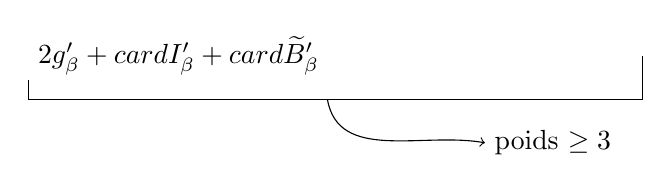
\begin{tikzpicture}[x=1cm,y=1cm]
\node[anchor=west] at (0,0) {$2g'_\beta+\operatorname{card}I'_\beta+\operatorname{card}\widetilde B'_\beta$};
\draw (0,-0.3)--(0,-0.55)--(7.8,-0.55)--(7.8,0);
\draw[->] (3.8,-0.55) to[out=-80,in=170] (5.8,-1.1);
\node[anchor=west] at (5.8,-1.1) {poids $\geq3$};
\end{tikzpicture}}}

\deleted{\unsure{qui a priori} \unsure{$+\operatorname{car}$} $\left[2g'_\beta+\operatorname{card}I'_\beta\geq3\right]$ $2g'_\beta+\operatorname{card}I'_\beta+\operatorname{card}\widetilde A'_\beta\geq3)$ qui a priori est une condition plus faible (puisque $\underline G'$ est un MD-graphe)\ldots}

d) le genre du MD-graphe $\underline G(\alpha)$ est égal à $g_\alpha$, i.e. on a
\[
\sum_{\beta\in S'_\alpha}\unsure{g'_\beta|\gamma'_\beta}+h_1(G(\alpha))=g_\alpha.
\]
\mspage{39}
